% !Mode:: "TeX:UTF-8"
% !TEX program  = xelatex

\documentclass[bwprint]{report}

\title{西南交大校园论坛系统部署手册}
\stunum{11}
\stuname{{程泽凯、金井直、赵祺、蒋焰}}
\dateinput{\today}
\def\makeothertitle{}
\setlength{\cftsecnumwidth}{3.2em}
\setlength{\cftsubsecnumwidth}{4.4em}
\setlength{\cftsubsubsecnumwidth}{5.6em}

\begin{document}

\maketitle
\newpage

\pagestyle{plain}
\pagenumbering{Roman}
\begin{center}
    {\zihao{4}\bfseries 摘要}
\end{center}

本文档面向西南交大校园论坛系统的实际部署需求，提供从本地开发环境搭建到阿里云生产环境上线的完整操作指南。系统采用前后端分离架构，前端基于 Vite 多页面应用（MPA）构建，后端基于 Spring Boot 3.2 实现业务逻辑与 REST API，数据库使用 MySQL 8。本文档覆盖环境准备、数据库初始化、后端构建部署、前端构建部署、Nginx 反向代理配置、systemd 服务托管和上线后验证等环节，并针对 Windows 本地开发与 Linux 服务器生产两种场景分别给出详细步骤。文档中的端口规划、命令示例和配置文件均来源于项目实际部署经验，可直接用于指导系统上线。

\vspace{0.5em}
\noindent{\heiti 关键词：}校园论坛；Spring Boot；Vite；Nginx；MySQL；Linux 部署

\newpage
\tableofcontents
\newpage
\pagestyle{plain}

\setcounter{page}{1}
\pagenumbering{arabic}

\section{项目概述}

\subsection{系统简介}

西南交大校园论坛是一个面向校园场景的综合社区系统，围绕"浏览、发帖、评论、互动、圈子、成长、积分、内容治理、运营管理"构建完整的前后端功能闭环。系统支持普通用户、版主和管理员三类角色，涵盖以下核心功能模块：

\begin{itemize}
    \item 账号认证：用户注册、JWT 登录鉴权、角色权限控制
    \item 首页信息流：最新/最热排序、帖子列表、校园热词云
    \item 发帖系统：标题、正文、板块、标签、多图上传（最多 9 张）
    \item 帖子详情：正文查看、评论、点赞、收藏、举报
    \item 用户主页：个人资料、等级徽章、发帖列表、关注管理
    \item 圈子系统：浏览、加入、创建圈子，按圈子筛选帖子
    \item 成长中心：每日签到、积分流水、等级成长、徽章展示
    \item 积分商城：商品浏览兑换（普通用户）、上架下架（管理员）
    \item 通知系统：评论、点赞、收藏、系统通知
    \item 内容治理：举报处理、帖子审核、内容审核记录
    \item 用户管理：用户状态管理、角色调整、账号禁用恢复
    \item 数据看板：后台总览统计、趋势分析、运营指标
\end{itemize}

\subsection{技术栈}

\begin{table}[H]
    \caption{系统技术栈}
    \label{tab:tech-stack}
    \centering
    \begin{tabular}{lc}
        \toprule[1.5pt]
        层级 & 技术 \\
        \midrule[1pt]
        前端框架 & Vite 5、多页面应用（MPA）、HTML、CSS、JavaScript ES Modules \\
        后端框架 & Java 17、Spring Boot 3.2、Spring MVC、Spring Security \\
        数据持久化 & Spring Data JPA、MySQL 8 \\
        鉴权方案 & JWT Bearer Token、角色权限控制 \\
        构建工具 & Maven、npm、Vite \\
        部署方案 & Linux + systemd + Nginx + MySQL \\
        \bottomrule[1.5pt]
    \end{tabular}
\end{table}

\subsection{项目结构}

项目核心目录结构如下：

\begin{lstlisting}
swjtu-forum/
├── backend/                         # Spring Boot 后端
│   ├── src/main/java/com/swjtu/forum/
│   │   ├── config/                  # 跨域、启动数据、Web 配置
│   │   ├── controller/              # REST API 控制器
│   │   ├── service/                 # 业务服务层
│   │   ├── repository/              # JPA Repository
│   │   ├── entity/                  # JPA 实体
│   │   ├── security/                # JWT 认证与安全配置
│   │   ├── dto/                     # 请求/响应 DTO
│   │   └── exception/               # 全局异常处理
│   ├── src/main/resources/
│   │   ├── application.yml          # 默认配置（H2 模式）
│   │   ├── application-mysql.yml    # MySQL 部署配置
│   │   ├── application-demo.yml     # 演示数据配置
│   │   └── schema.sql               # 数据库结构脚本
│   └── pom.xml
├── frontend/                        # Vite 多页面前端
│   ├── assets/                      # 共享资源（API、样式、动画）
│   ├── home_recommended/            # 首页
│   ├── login_register/              # 登录注册
│   ├── create_post/                 # 发帖
│   ├── post_details/                # 帖子详情
│   ├── admin_overview/              # 管理后台
│   ├── ...                          # 其他页面模块
│   └── vite.config.js
├── docs/                            # 设计文档与 API 文档
├── init-database.sql                # MySQL 数据库初始化脚本
├── start.ps1                        # Windows 一键启动脚本
└── README.md                        # 项目说明文档
\end{lstlisting}

\begin{figure}[H]
    \centering
    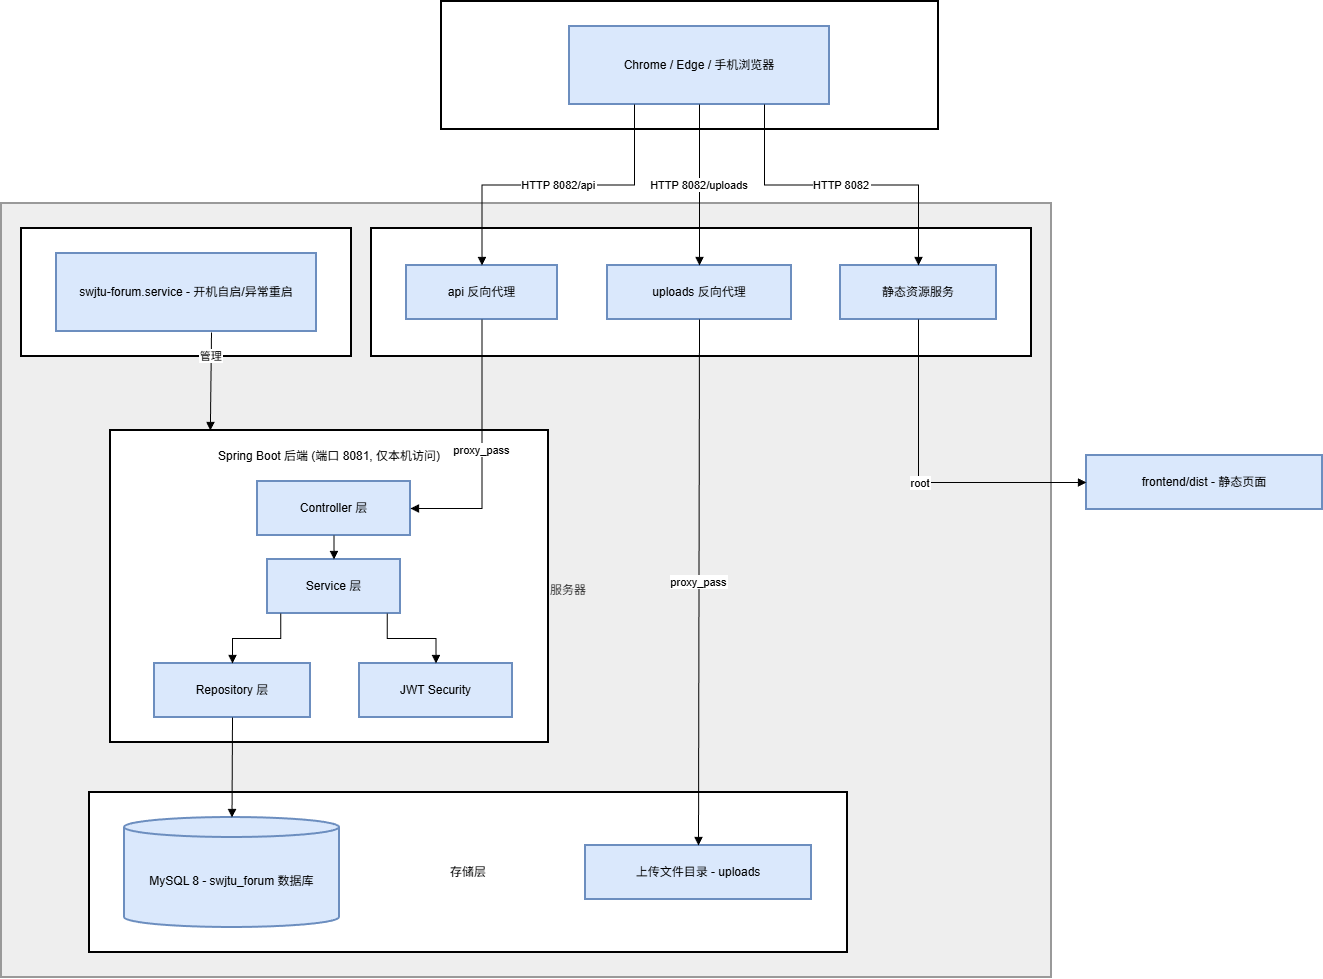
\includegraphics[width=0.85\textwidth]{figures/system_architecture.png}
    \caption{系统部署架构图}
    \label{fig:architecture}
\end{figure}

\section{环境要求}

\subsection{硬件要求}

\begin{table}[H]
    \caption{推荐硬件配置}
    \label{tab:hardware}
    \centering
    \begin{tabular}{lcc}
        \toprule[1.5pt]
        环境 & CPU & 内存 \\
        \midrule[1pt]
        本地开发 & 4 核及以上 & 8 GB 及以上 \\
        服务器（阿里云轻量） & 2 核 & 4 GB \\
        便携演示包 & 4 核及以上 & 8 GB 及以上 \\
        \bottomrule[1.5pt]
    \end{tabular}
\end{table}

\subsection{软件环境}

\subsubsection{本地开发环境（Windows）}

\begin{itemize}
    \item 操作系统：Windows 10/11 或 Windows Server 2019+
    \item Java 17（JDK 17，推荐 Eclipse Temurin 或 Oracle JDK 17）
    \item Maven 3.9+（用于后端构建）
    \item Node.js 18+ / npm 9+（用于前端构建）
    \item MySQL 8.0+（可选，正式部署推荐）
    \item Redis 6/7（可选，缓存增强）
    \item Git（用于版本管理）
\end{itemize}

\subsubsection{服务器环境（Linux）}

\begin{itemize}
    \item 操作系统：Ubuntu 22.04 LTS（阿里云轻量应用服务器已验证）
    \item Java 17（openjdk-17-jdk）
    \item Maven 3.9+
    \item Node.js 20（LTS）
    \item MySQL 8.0+
    \item Nginx（最新稳定版）
    \item systemd（服务托管）
    \item Git
\end{itemize}

\begin{figure}[H]
    \centering
    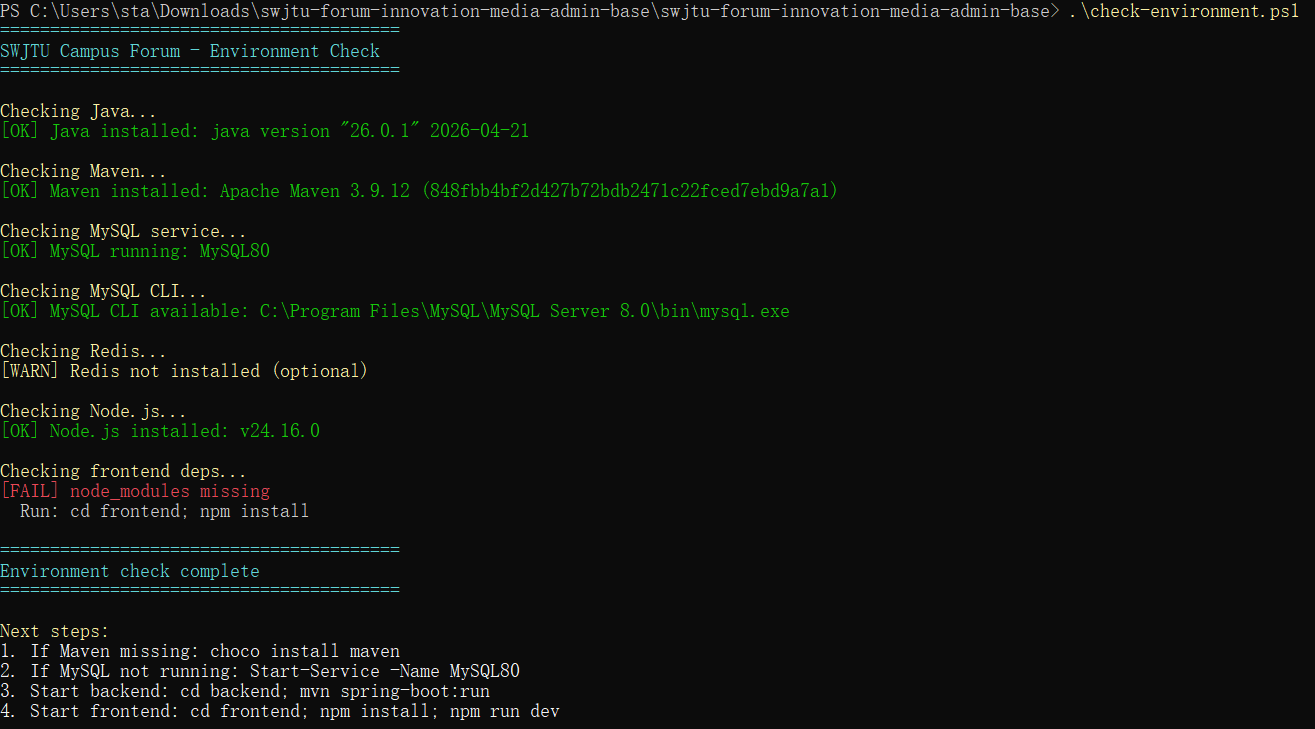
\includegraphics[width=0.8\textwidth]{figures/env_check.png}
    \caption{环境检查结果示例}
    \label{fig:env-check}
\end{figure}

\section{本地部署（Windows）}

\subsection{环境准备}

\subsubsection{安装 Java 17}

从 Adoptium 官网下载 JDK 17（\texttt{https://adoptium.net}），安装后配置系统环境变量：

\begin{lstlisting}
# 验证安装
java -version
# 期望输出：openjdk version "17.0.x"
\end{lstlisting}

\subsubsection{安装 Maven}

从 Maven 官网下载（\texttt{https://maven.apache.org/download.cgi}），解压后配置 \texttt{MAVEN\_HOME} 环境变量：

\begin{lstlisting}
# 验证安装
mvn -version
# 期望输出：Apache Maven 3.9.x
\end{lstlisting}

\subsubsection{安装 Node.js}

从 Node.js 官网下载 18+ LTS 版本（\texttt{https://nodejs.org}），安装后验证：

\begin{lstlisting}
node -v   # 期望输出：v18.x.x 或 v20.x.x
npm -v    # 期望输出：9.x.x 或 10.x.x
\end{lstlisting}

\subsubsection{安装 MySQL 8}

从 MySQL 官网下载安装包，安装过程中设置 root 密码。建议将 MySQL 安装目录的 \texttt{bin} 路径加入系统 PATH。

\subsection{数据库初始化}

\subsubsection{方式一：使用一键初始化脚本}

在项目根目录执行：

\begin{lstlisting}
mysql -u root -p < init-database.sql
\end{lstlisting}

输入 root 密码后，脚本将自动创建 \texttt{swjtu\_forum} 数据库，字符集为 \texttt{utf8mb4}，排序规则为 \texttt{utf8mb4\_unicode\_ci}。

\subsubsection{方式二：手动创建}

启动 MySQL 服务后，登录 MySQL 客户端手动执行：

\begin{lstlisting}
CREATE DATABASE IF NOT EXISTS swjtu_forum
  CHARACTER SET utf8mb4
  COLLATE utf8mb4_unicode_ci;

CREATE USER IF NOT EXISTS 'swjtu_forum'@'localhost'
  IDENTIFIED BY 'your-strong-password';

GRANT ALL PRIVILEGES ON swjtu_forum.* TO 'swjtu_forum'@'localhost';
FLUSH PRIVILEGES;
EXIT;
\end{lstlisting}

\subsection{一键启动（推荐）}

项目根目录提供了 \texttt{start.ps1} 一键启动脚本，自动完成端口清理、依赖检查、后端构建和前端构建步骤。

\subsubsection{MySQL 模式启动}

\begin{lstlisting}
# 设置环境变量（替换为实际值）
$env:DB_USERNAME = "root"
$env:DB_PASSWORD = "your-mysql-password"
$env:JWT_SECRET = "your-long-random-secret-at-least-32-chars"

# 执行一键启动
.\start.ps1
\end{lstlisting}

脚本自动执行以下步骤：

\begin{enumerate}
    \item 清理本地 8080 / 4173 端口的残留进程
    \item 检查 \texttt{node\_modules}，缺失时自动执行 \texttt{npm install}
    \item 检查后端 JAR 包，缺失或过期时自动用 Maven 重新构建
    \item 重新构建前端 \texttt{dist} 目录
    \item 启动 Spring Boot 后端（MySQL 模式）
    \item 启动 Vite Preview 前端服务器
    \item 轮询后端健康检查接口，确认服务可用
    \item 打印前端访问地址和默认管理员账号
\end{enumerate}

启动成功后输出：

\begin{lstlisting}
============================================================
 All services are ready!
------------------------------------------------------------
 Frontend  : http://localhost:4173
 Backend   : http://localhost:8080/api
 Database  : MySQL profile, database name swjtu_forum
------------------------------------------------------------
 Default admin: admin / admin123456
============================================================
\end{lstlisting}

\begin{figure}[H]
    \centering
    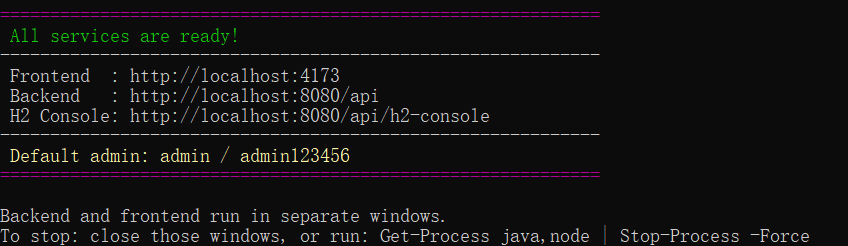
\includegraphics[width=0.85\textwidth]{figures/start_script_success.png}
    \caption{一键启动脚本运行成功界面}
    \label{fig:start-script}
\end{figure}

\subsection{手动分步启动}

若需要手动控制启动流程，可按照以下步骤操作。

\subsubsection{后端手动启动}

\begin{lstlisting}
cd backend

# 设置环境变量
$env:DB_URL = "jdbc:mysql://127.0.0.1:3306/swjtu_forum?useUnicode=true&characterEncoding=utf8&useSSL=false&serverTimezone=Asia/Shanghai&allowPublicKeyRetrieval=true"
$env:DB_USERNAME = "root"
$env:DB_PASSWORD = "your-mysql-password"
$env:JWT_SECRET = "your-long-random-secret-at-least-32-chars"

# 使用 Maven 直接运行
mvn spring-boot:run -Dspring-boot.run.profiles=mysql
\end{lstlisting}

后端启动后在 \texttt{http://localhost:8080/api} 提供 REST 接口。首次启动时 Spring Data JPA 会自动根据实体类同步数据库表结构，同时 Java Seeder 自动写入基础管理员账号、版块数据和演示帖子。

\subsubsection{前端手动启动}

\begin{lstlisting}
cd frontend
npm install        # 首次启动或依赖更新时运行
npm run dev        # 开发模式，默认端口 5173，支持热更新
\end{lstlisting}

Vite 开发服务器会自动将 \texttt{/api} 请求代理到后端 \texttt{http://localhost:8080}。

\subsubsection{生产构建模式}

\begin{lstlisting}
cd frontend
npm run build      # 构建生产版本，输出到 frontend/dist/
npm run preview    # 预览构建产物，默认端口 4173
\end{lstlisting}

\subsection{H2 演示模式（免 MySQL）}

若当前环境没有安装 MySQL，可以使用 H2 内存数据库模式快速启动：

\begin{lstlisting}
.\start.ps1 -SpringProfile demo
\end{lstlisting}

该模式下：
\begin{itemize}
    \item 使用 H2 文件数据库，无需安装 MySQL
    \item 自动创建演示数据（用户、帖子、评论等）
    \item H2 控制台地址：\texttt{http://localhost:8080/api/h2-console}
    \item JDBC URL：\texttt{jdbc:h2:file:./data/swjtu-forum-demo}
    \item 注意：该模式仅适合本地演示和开发调试，不推荐用于生产环境
\end{itemize}

\begin{figure}[H]
    \centering
    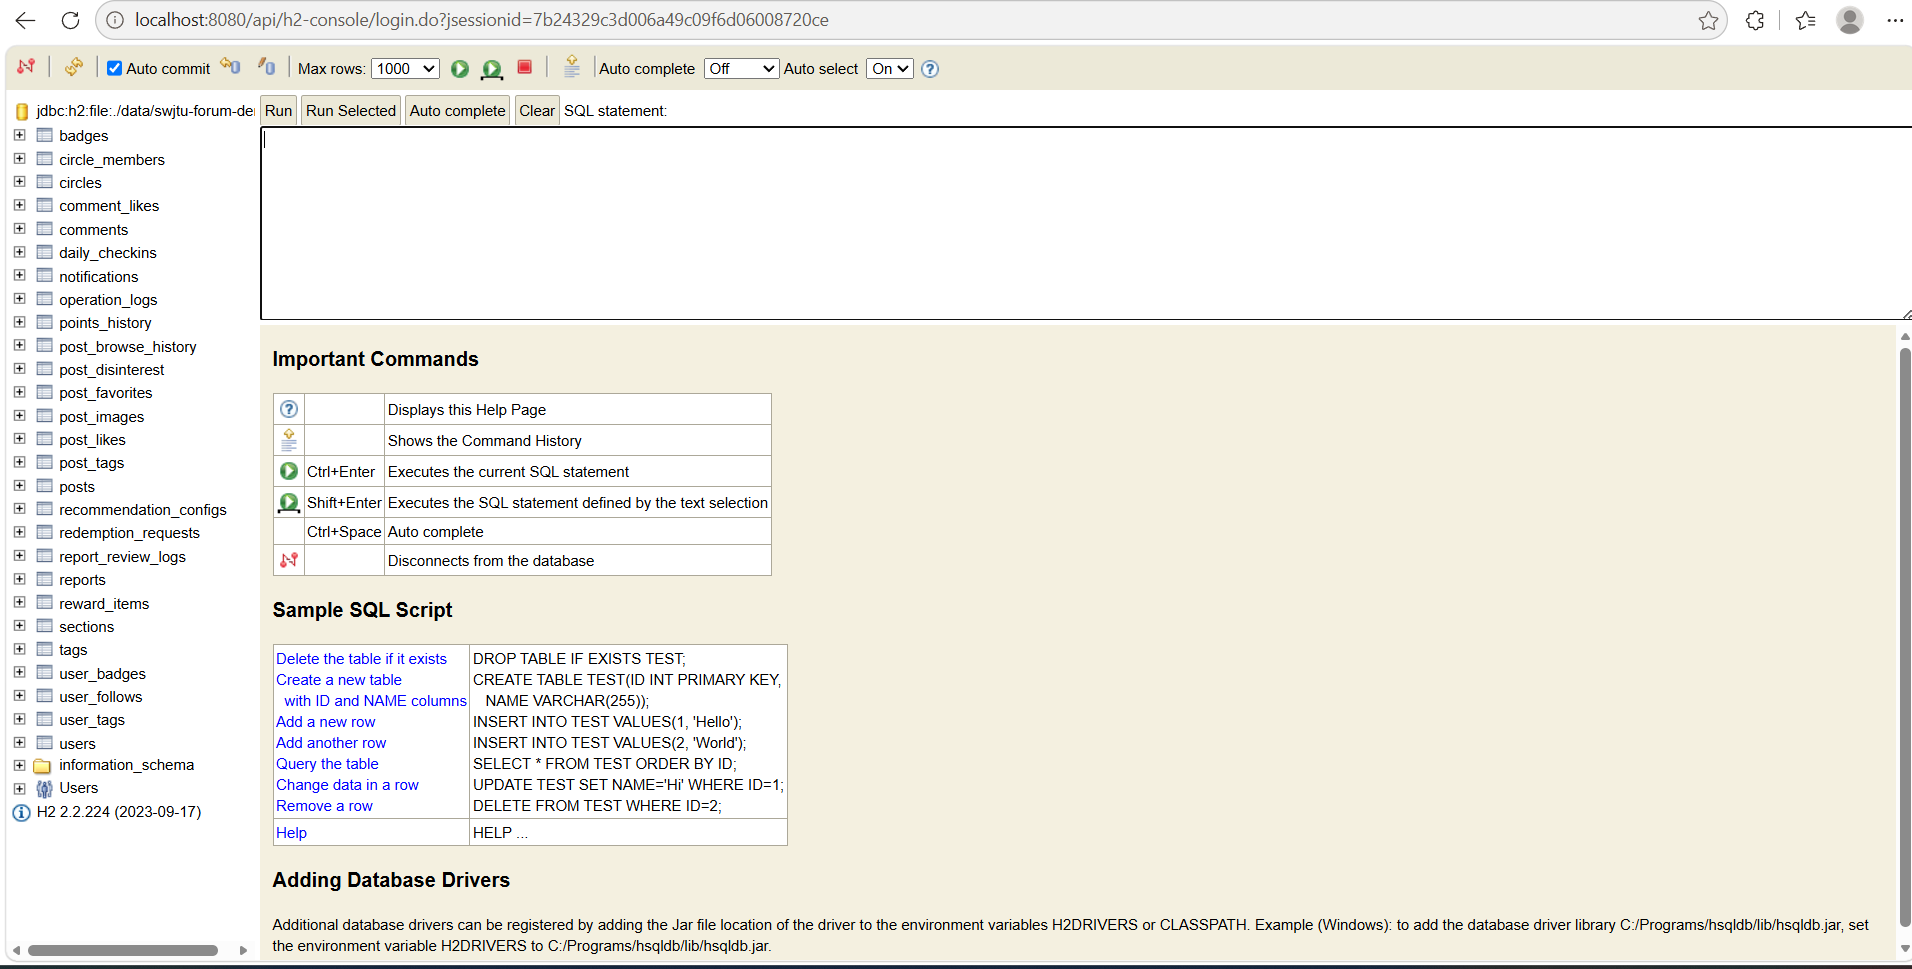
\includegraphics[width=0.7\textwidth]{figures/h2_console.png}
    \caption{H2 数据库控制台登录界面}
    \label{fig:h2-console}
\end{figure}

\subsection{环境检查工具}

项目提供了环境检查脚本，可快速确认当前机器是否满足运行条件：

\begin{lstlisting}
.\check-environment.ps1
\end{lstlisting}

脚本依次检查 Java、Maven、MySQL 服务、MySQL CLI、Redis 和 Node.js 的安装状态，并给出缺失提示和安装建议。

\section{服务器部署（Linux）}

本章基于 Ubuntu 22.04 LTS 阿里云轻量应用服务器编写。部署目标是在不干扰服务器上已有服务的前提下，为论坛分配独立端口并完成上线。

\subsection{端口规划}

为与服务器上已有的 80 端口网站共存，论坛采用如下端口规划：

\begin{table}[H]
    \caption{服务器端口规划}
    \label{tab:port-plan}
    \centering
    \begin{tabular}{lccc}
        \toprule[1.5pt]
        服务 & 端口 & 暴露范围 & 说明 \\
        \midrule[1pt]
        原网站 Nginx & 80 & 公网 & 保持不动 \\
        原有后端 & 8000 & 127.0.0.1 & 原有服务不变 \\
        论坛前端入口 & 8082 & 公网 & Nginx 监听，浏览器访问 \\
        论坛后端 & 8081 & 127.0.0.1 & Spring Boot，仅 Nginx 反代 \\
        MySQL & 3306 & 本机 & 数据库存储 \\
        SSH & 22 & 公网 & 远程管理 \\
        \bottomrule[1.5pt]
    \end{tabular}
\end{table}

 
\subsection{安装基础环境}

登录到服务器后，依次执行以下命令安装所需软件包：

\begin{lstlisting}
# 更新软件包索引
sudo apt update

# 安装基础工具
sudo apt install -y git curl wget unzip nginx mysql-server maven openjdk-17-jdk
\end{lstlisting}

\subsubsection{安装 Node.js 20}

\begin{lstlisting}
curl -fsSL https://deb.nodesource.com/setup_20.x | sudo -E bash -
sudo apt install -y nodejs
node -v    # 验证安装
npm -v
\end{lstlisting}

注意：Vite 5 要求 Node.js 18 或更高版本。若服务器原本安装了旧版 Node.js，可能需要先卸载：

\begin{lstlisting}
sudo apt remove -y nodejs libnode-dev
sudo apt --fix-broken install -y
curl -fsSL https://deb.nodesource.com/setup_20.x | sudo -E bash -
sudo apt install -y nodejs
\end{lstlisting}

\subsection{数据库初始化}

创建独立数据库用户和数据库（不直接使用 root）：

\begin{lstlisting}
sudo mysql
\end{lstlisting}

在 MySQL 提示符下执行：

\begin{lstlisting}
CREATE DATABASE IF NOT EXISTS swjtu_forum
  CHARACTER SET utf8mb4
  COLLATE utf8mb4_unicode_ci;

CREATE USER IF NOT EXISTS 'swjtu_forum'@'localhost'
  IDENTIFIED BY 'your-strong-password';

GRANT ALL PRIVILEGES ON swjtu_forum.* TO 'swjtu_forum'@'localhost';
FLUSH PRIVILEGES;
EXIT;
\end{lstlisting}

\subsection{拉取项目代码}

\begin{lstlisting}
# 首次部署
sudo mkdir -p /opt/swjtu-forum
sudo chown -R $USER:$USER /opt/swjtu-forum
git clone -b innovation/media-admin-base
  https://gitee.com/czk2370708935/swjtu-forum.git
  /opt/swjtu-forum
\end{lstlisting}

后续更新：

\begin{lstlisting}
cd /opt/swjtu-forum
git pull origin innovation/media-admin-base
\end{lstlisting}

\subsection{构建后端}

\begin{lstlisting}
cd /opt/swjtu-forum/backend
mvn clean package -DskipTests
\end{lstlisting}

构建成功后生成：

\begin{lstlisting}
/opt/swjtu-forum/backend/target/forum-1.0.0.jar
\end{lstlisting}

\begin{figure}[H]
    \centering
    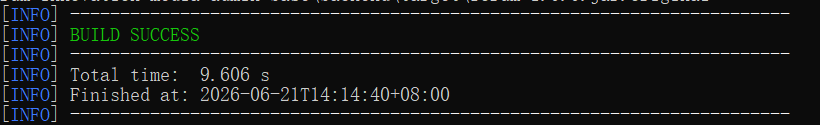
\includegraphics[width=0.85\textwidth]{figures/maven_build_success.png}
    \caption{后端 Maven 构建成功}
    \label{fig:maven-build}
\end{figure}

\subsection{配置 systemd 服务}

创建 systemd 服务文件，使后端以系统服务方式运行，支持开机自启和异常自动重启。

\begin{lstlisting}
sudo nano /etc/systemd/system/swjtu-forum.service
\end{lstlisting}

写入以下内容（替换数据库密码和 JWT 密钥）：

\begin{lstlisting}
[Unit]
Description=SWJTU Forum Backend
After=network.target mysql.service

[Service]
WorkingDirectory=/opt/swjtu-forum/backend
ExecStart=/usr/bin/java -Dfile.encoding=UTF-8
  -Dspring.profiles.active=mysql
  -jar /opt/swjtu-forum/backend/target/forum-1.0.0.jar
  --server.port=8081
Environment=DB_URL=jdbc:mysql://127.0.0.1:3306/swjtu_forum
  ?useUnicode=true&characterEncoding=utf8
  &useSSL=false&serverTimezone=Asia/Shanghai
  &allowPublicKeyRetrieval=true
Environment=DB_USERNAME=swjtu_forum
Environment=DB_PASSWORD=your-db-password
Environment=JWT_SECRET=your-long-random-secret-at-least-32-chars
Environment=APP_CORS_ALLOWED_ORIGIN_PATTERNS=
  http://your-server-ip:8082
Restart=always
RestartSec=5

[Install]
WantedBy=multi-user.target
\end{lstlisting}

启动服务：

\begin{lstlisting}
sudo systemctl daemon-reload
sudo systemctl enable --now swjtu-forum
sudo systemctl status swjtu-forum
\end{lstlisting}

查看实时日志：

\begin{lstlisting}
sudo journalctl -u swjtu-forum -f
\end{lstlisting}

 
\subsection{构建前端}

\begin{lstlisting}
cd /opt/swjtu-forum/frontend
npm install
npm run build
\end{lstlisting}

构建产物位于 \texttt{/opt/swjtu-forum/frontend/dist} 目录。

\subsection{配置 Nginx}

创建 Nginx 站点配置文件：

\begin{lstlisting}
sudo nano /etc/nginx/conf.d/swjtu-forum.conf
\end{lstlisting}

写入配置：

\begin{lstlisting}
server {
    listen 8082;
    server_name _;

    root /opt/swjtu-forum/frontend/dist;
    index index.html;

    # 反向代理 API 请求到后端
    location /api/ {
        proxy_pass http://127.0.0.1:8081/api/;
        proxy_set_header Host $host;
        proxy_set_header X-Real-IP $remote_addr;
        proxy_set_header X-Forwarded-For
          $proxy_add_x_forwarded_for;
    }

    # 反向代理上传文件请求
    location /uploads/ {
        proxy_pass http://127.0.0.1:8081/uploads/;
    }

    # 前端静态资源
    location / {
        try_files $uri $uri/ /index.html;
    }
}
\end{lstlisting}

检查配置并重载 Nginx：

\begin{lstlisting}
sudo nginx -t
sudo systemctl reload nginx
\end{lstlisting}

 
\subsection{配置防火墙}

在阿里云轻量应用服务器控制台中，添加防火墙规则：

\begin{table}[H]
    \caption{云服务器防火墙规则}
    \label{tab:firewall-rules}
    \centering
    \begin{tabular}{lccc}
        \toprule[1.5pt]
        协议 & 端口 & 来源 & 说明 \\
        \midrule[1pt]
        TCP & 22 & 0.0.0.0/0 & SSH 远程管理 \\
        TCP & 80 & 0.0.0.0/0 & 原网站（保留） \\
        TCP & 443 & 0.0.0.0/0 & HTTPS（可选） \\
        TCP & 8082 & 0.0.0.0/0 & 论坛公网访问入口 \\
        \bottomrule[1.5pt]
    \end{tabular}
\end{table}

注意：8081 是后端内部端口，仅 Nginx 通过本机网络访问，不需要在公网防火墙开放。

若服务器启用了 UFW，也需要放行：

\begin{lstlisting}
sudo ufw allow 8082/tcp
sudo ufw status
\end{lstlisting}

\section{部署验证}

\subsection{本地服务检查}

\begin{lstlisting}
# 检查前端静态资源是否正常
curl -I http://127.0.0.1:8082/

# 检查后端 API 是否可用
curl -i http://127.0.0.1:8082/api/sections

# 检查公网访问是否正常
curl -I http://your-server-ip:8082/
\end{lstlisting}

\subsection{功能验收清单}

部署完成后，建议逐项验证以下功能：

\begin{table}[H]
    \caption{部署验收测试用例}
    \label{tab:verification}
    \centering
    \small
    \begin{tabular}{p{0.08\textwidth}p{0.28\textwidth}p{0.28\textwidth}p{0.2\textwidth}}
        \toprule[1.5pt]
        编号 & 测试项 & 操作步骤 & 预期结果 \\
        \midrule[1pt]
        T-01 & 页面访问 & 浏览器打开 \texttt{http://IP:8082} & 首页正常加载，板块、热词可见 \\
        T-02 & 用户注册 & 注册新用户 & 注册成功并可登录 \\
        T-03 & 管理员登录 & 使用 \texttt{admin/admin123456} 登录 & 可进入管理后台 \\
        T-04 & 发帖功能 & 登录后发布图文帖子 & 帖子出现在首页列表中 \\
        T-05 & 评论点赞 & 在详情页评论并点赞 & 评论展示，点赞状态更新 \\
        T-06 & 图片上传 & 上传 PNG/JPG 图片 & 图片正常显示，不超 9 张 \\
        T-07 & 签到功能 & 进入成长中心签到 & 获得积分，按钮置灰 \\
        T-08 & 内容治理 & 管理员处理举报 & 帖子状态更新 \\
        T-09 & CORS 验证 & 公网访问 API & 不出现 403 CORS 错误 \\
        T-10 & 后台数据 & 管理员查看数据看板 & 统计信息正常加载 \\
        \bottomrule[1.5pt]
    \end{tabular}
\end{table}

\subsection{常见问题排查}

\begin{table}[H]
    \caption{常见部署问题与解决方案}
    \label{tab:troubleshooting}
    \centering
    \small
    \begin{tabular}{p{0.25\textwidth}p{0.25\textwidth}p{0.35\textwidth}}
        \toprule[1.5pt]
        问题 & 可能原因 & 解决方案 \\
        \midrule[1pt]
        注册接口 403 & CORS 配置未包含公网地址 & 修改 \texttt{APP\_CORS\_ALLOWED\_ORIGIN\_PATTERNS} 环境变量，重启后端 \\
        502 Bad Gateway & Nginx 无法连接后端 & 检查 \texttt{sudo systemctl status swjtu-forum}，确认后端运行在 8081 端口 \\
        图片不显示 & 上传目录代理缺失 & 检查 Nginx 配置中 \texttt{/uploads/} 代理和后端目录权限 \\
        前端白屏 & 构建缓存或配置错误 & 重新构建前端，清理浏览器缓存，检查 Nginx root 路径 \\
        数据库连接失败 & 账号密码或网络错误 & 确认 MySQL 服务运行、账号权限正确、\texttt{DB\_URL} 配置无误 \\
        npm 构建失败 & Node.js 版本过低 & 升级至 Node.js 18 或 20（Vite 5 不支持 Node 12） \\
        端口被占用 & 其他进程占用端口 & 使用 \texttt{sudo ss -tulpn | grep 端口号} 查看冲突进程 \\
        \bottomrule[1.5pt]
    \end{tabular}
\end{table}

\section{便携交付包部署}

项目支持生成便携交付包，适合发给老师或同学直接运行，不依赖 MySQL、Node.js 和 Maven。

\subsection{生成便携包}

在项目根目录执行：

\begin{lstlisting}
.\build-portable.ps1
\end{lstlisting}

\begin{figure}[H]
    \centering
    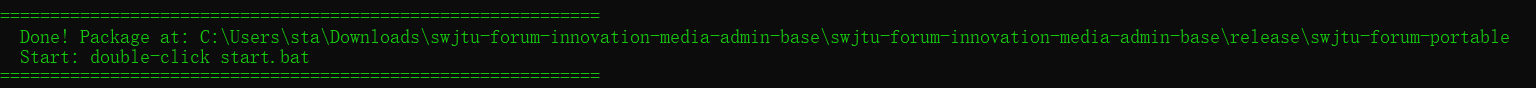
\includegraphics[width=0.85\textwidth]{figures/portable_build.png}
    \caption{便携交付包构建过程}
    \label{fig:portable-build}
\end{figure}

构建过程包含以下步骤：

\begin{enumerate}
    \item 使用 Maven 构建后端 JAR 包
    \item 使用 npm 构建前端 dist 目录
    \item 使用 jlink 生成最小化 JRE（仅包含后端运行所需模块）
    \item 编译静态前端服务器（FrontendServer.java）
    \item 将后端 JAR、前端 dist、JRE 和启动脚本打包到 \texttt{release/swjtu-forum-portable/}
\end{enumerate}

输出目录结构：

\begin{lstlisting}
release/swjtu-forum-portable/
├── app/
│   ├── backend/
│   │   └── forum-1.0.0.jar        # 后端可执行 JAR
│   └── frontend/
│       └── dist/                   # 前端构建产物
├── runtime/                        # 最小化 JRE
├── start.bat                       # 启动脚本（Windows）
├── stop.bat                        # 停止脚本
├── start-portable.ps1              # PowerShell 启动脚本
└── README.txt                      # 使用说明
\end{lstlisting}

\subsection{运行便携包}

\begin{lstlisting}
# 方式一：双击 start.bat（推荐）
# 方式二：在 release/swjtu-forum-portable/ 目录执行
.\start-portable.ps1
\end{lstlisting}

便携包使用以下默认配置：

\begin{itemize}
    \item 后端端口：8080
    \item 前端端口：4173
    \item Spring Profile：demo（H2 文件数据库）
    \item 数据文件路径：\texttt{app/backend/data/swjtu-forum-demo.mv.db}
    \item 默认管理员：\texttt{admin / admin123456}
\end{itemize}

若端口冲突，可指定其他端口：

\begin{lstlisting}
.\start-portable.ps1 -BackendPort 8081 -FrontendPort 4174
\end{lstlisting}

\section{系统维护}

\subsection{后端更新流程}

\begin{lstlisting}
cd /opt/swjtu-forum
git pull origin innovation/media-admin-base
cd backend
mvn clean package -DskipTests
sudo systemctl restart swjtu-forum
sudo systemctl status swjtu-forum
\end{lstlisting}

\subsection{前端更新流程}

\begin{lstlisting}
cd /opt/swjtu-forum/frontend
npm install
npm run build
sudo nginx -t
sudo systemctl reload nginx
\end{lstlisting}

\subsection{数据库备份}

\begin{lstlisting}
# 导出数据库
mysqldump -u swjtu_forum -p swjtu_forum > backup_$(date +%Y%m%d).sql

# 还原数据库
mysql -u swjtu_forum -p swjtu_forum < backup_20260601.sql
\end{lstlisting}

\subsection{日志管理}

\begin{lstlisting}
# 查看后端实时日志
sudo journalctl -u swjtu-forum -f

# 查看 Nginx 访问日志
sudo tail -f /var/log/nginx/access.log

# 查看 Nginx 错误日志
sudo tail -f /var/log/nginx/error.log
\end{lstlisting}

\subsection{安全建议}

\begin{itemize}
    \item 上线后立即修改默认管理员密码，避免使用 \texttt{admin123456}
    \item 禁止将数据库密码和 JWT 密钥提交到 Git 仓库
    \item 定期更新服务器软件包：\texttt{sudo apt update \&\& sudo apt upgrade}
    \item 开启 MySQL 的 \texttt{binlog} 以便数据恢复
    \item 上传目录定期清理，防止磁盘占满
    \item 仅开放必要端口，后端 8081 端口限制为本机访问
\end{itemize}

\section{附录}

\subsection{默认账号信息}

\begin{table}[H]
    \caption{系统默认账号}
    \label{tab:default-accounts}
    \centering
    \begin{tabular}{lccc}
        \toprule[1.5pt]
        账号 & 密码 & 角色 & 说明 \\
        \midrule[1pt]
        admin & admin123456 & 管理员 & 后台管理、用户管理、内容治理 \\
        \bottomrule[1.5pt]
    \end{tabular}
\end{table}

普通用户可从前端注册页面自行注册。

\subsection{环境变量说明}

\begin{table}[H]
    \caption{后端环境变量}
    \label{tab:env-vars}
    \centering
    \small
    \begin{tabular}{lll}
        \toprule[1.5pt]
        变量名 & 说明 & 默认值 \\
        \midrule[1pt]
        \texttt{DB\_URL} & MySQL 连接 URL & \texttt{jdbc:mysql://localhost:3306/swjtu\_forum?...} \\
        \texttt{DB\_USERNAME} & 数据库用户名 & root \\
        \texttt{DB\_PASSWORD} & 数据库密码 & 空 \\
        \texttt{JWT\_SECRET} & JWT 签名密钥 & 内置开发用默认值 \\
        \texttt{JWT\_EXPIRATION} & Token 过期时间（ms） & 86400000（24 小时） \\
        \texttt{SERVER\_PORT} & 后端监听端口 & 8080 \\
        \texttt{REDIS\_HOST} & Redis 主机 & localhost \\
        \texttt{REDIS\_PORT} & Redis 端口 & 6379 \\
        \texttt{APP\_CORS\_ALLOWED\_ORIGIN\_PATTERNS} & 允许的跨域来源 & 本地地址 \\
        \texttt{DEMO\_SEED\_ENABLED} & 是否写入演示数据 & true \\
        \bottomrule[1.5pt]
    \end{tabular}
\end{table}

\subsection{常用命令速查}

\begin{lstlisting}
# 后端
cd backend && mvn spring-boot:run                   # 开发运行
cd backend && mvn test                              # 运行测试
cd backend && mvn clean package -DskipTests          # 打包 JAR

# 前端
cd frontend && npm install                          # 安装依赖
cd frontend && npm run dev                          # 开发模式
cd frontend && npm run build                        # 生产构建
cd frontend && npm test                             # 运行测试

# 运维
sudo systemctl start|stop|restart|status swjtu-forum # 后端服务管理
sudo journalctl -u swjtu-forum -f                   # 查看后端日志
sudo nginx -t                                       # 检查 Nginx 配置
sudo systemctl reload nginx                         # 重载 Nginx
sudo systemctl reload nginx                         # 重载防火墙
\end{lstlisting}

\end{document}
